% !TeX root = ../main.tex
\chapter{研究Casimir效应的基本理论}
\section{半经典理论}
在量子场论中,可以用简谐振子模型将电磁场量子化,量子化后的零点能为:
$$
E_0=\sum_k{\frac{1}{2} \hbar w_k}
$$
式中下标k表示系统允许的电磁场模态。考虑一个长,宽,高分别为L,L,a的由理想金属构成边界的腔体,如图\ref{fig:1}所示,系统允许存在的电磁场的波矢为:
$$
k_x=\frac{\pi}{L}n_x,k_y=\frac{\pi}{L}n_y,k_z=\frac{\pi}{a}n_z\left( n_x,n_y,n_z=0,1,2...... \right) 
$$
\begin{figure}[htb]
	\centering
	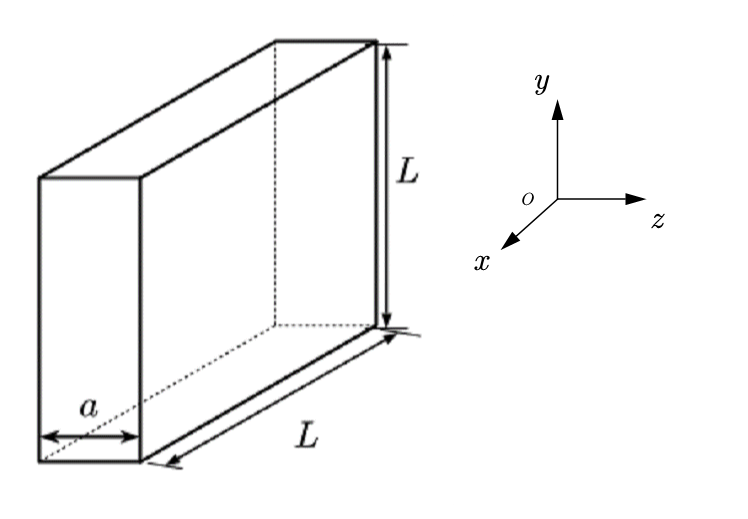
\includegraphics[width=0.7\linewidth]{figures/金属边界腔体}
	\caption{由理想金属构成边界的腔体}
	\label{fig:1}
\end{figure}
\paragraph*{}
电磁场的波矢大小可以写为:
$$
k=\sqrt{k_{x}^{2}+k_{y}^{2}+k_{z}^{2}}=\sqrt{\chi ^2+k_{z}^{2}}
$$
式中$\chi ^2=k_{x}^{2}+k_{y}^{2}$。当$n_x$,$n_y$,$n_z$全部非零时,$k_x$,$k_y$,$k_z$的取值对应于两种独立的振动模态;当$n_x$,$n_y$,$n_z$有一个为零时,$k_x$,$k_y$,$k_z$的取值对应于一种独立的振动模态;当$n_x$,$n_y$,$n_z$有两个或以上为零时,$k_x$,$k_y$,$k_z$的取值对应于零种独立的振动模态\cite{GuoShuohong_2008}。
\paragraph*{}
当L取很大值时对于$k_x$,$k_y$的求和可以转化为积分,当a取很大值时对于$k_z$的求和可以转化为积分,因此两个距离为a的金属板的相互作用能可以表示为:
\begin{equation*}
\begin{split}
\delta E &=\left. \sum_k{\frac{1}{2}\hbar w_k} \right|_{a=a} - \left. \sum_k{\frac{1}{2}\hbar w_k} \right|_{a\rightarrow \infty} \\
&= \hbar c\frac{L^2}{\pi ^2} \iint\limits_{k_x,k_y>0}^{} \left( \frac{1}{2}\sqrt{k_{x}^{2}+k_{y}^{2}}+\sum_{n=1}^{\infty}{\sqrt{n^2\frac{\pi ^2}{a^2}+k_{x}^{2}+k_{y}^{2}}} \right) dk_xdk_y  \\ 
&\quad - \hbar c\frac{L^2}{\pi ^2} \iiint\limits_{k_x,k_y,k_z>0}^{} \left( \sqrt{k_{z}^{2}+k_{x}^{2}+k_{y}^{2}} \right) dk_xdk_yd\left( \frac{a}{\pi}k_z \right) \\
&=\frac{\hbar cL^2}{2\pi}\left[ \sum_{\left( 0 \right) 1}^{\infty}{\int_0^{\infty}{\sqrt{n^2\frac{\pi ^2}{a^2}+\chi ^2}\cdot \chi d\chi -\iint\limits_{\chi ,k_z>0}^{}\sqrt{k_{z}^{2}+\chi ^2}\cdot \chi d\chi d\left( \frac{a}{\pi}k_z \right)}} \right]
\end{split}
\end{equation*}
式中$\sum\limits_{(0) 1}^{\infty}{}$表示对于n=0的一项求和时要乘以权重因子$\frac{1}{2}$,对于n$\geqslant$1项的求和,要乘以权重因子1,上式直接计算的结果是发散的,因此我们无法从中获取有效的物理信息。为了得到有限值结果,有必要给积分因子乘以一个加权函数$𝑓(𝑘/𝑘_𝑚 )$,它的特征是当$𝑘≪𝑘_𝑚$时值趋近于1,而当$𝑘≫𝑘_𝑚$时值趋近于0。这个函数的物理意义是对于波长非常短的波,金属的边界性条件不再成立,因此这一波段的电磁波不应包含在零点能的计算中。令$u=a^2\chi ^2/\pi ^2$,则有:
$$
\delta E=\frac{\hbar cL^2\pi ^2}{4a^3}\left[ \sum_{\left( 0 \right) 1}^{\infty}{\int_0^{\infty}{\sqrt{n^2+u}\cdot f\left( \frac{\pi \sqrt{n^2+u}}{ak_m} \right) du - \iint\limits_{n,u>0}^{} \sqrt{n^2+u}\cdot f\left( \frac{\pi \sqrt{n^2+u}}{ak_m} \right) dudn}} \right] 
$$
采用Euler-Maclaulin公式:
$$
\sum_{\left( 0 \right) 1}^{\infty}{F\left( n \right)}-\int_0^{\infty}{F\left( n \right) dn}=\frac{-1}{12}F'\left( 0 \right) +\frac{1}{720}F'''\left( 0 \right) +......
$$
取
\begin{equation*}
\begin{split}
F\left( n \right) &=\int_{n^2}^{\infty}{w^{1/2}f\left( \frac{w^{1/2}\pi}{ak_m} \right) dw} \\
F'\left( n \right) &=-2n^2f\left( \frac{w^{1/2}\pi}{ak_m} \right) ,F'\left( 0 \right) =0,F'''\left( 0 \right) =-4
\end{split}
\end{equation*}
则:
\begin{equation*}
\begin{split}
\delta E &=\frac{\hbar cL^2\pi ^2}{4a^3}\left( -\frac{1}{180} \right) =-\frac{\hbar cL^2\pi ^2}{720a^3}\\ 
F_c&=-\frac{\partial \left( \delta E \right)}{\partial a}=-\frac{\hbar cL^2\pi ^2}{240a^4}
\end{split}
\end{equation*}
至此我们便算出了单位面积理想导体平行板之间的Casimir力为$-\frac{\hbar c\pi ^2}{240a^4}$,式中负号代表两平行板间的Casimir力是吸引力。



\section{维度重整化法}
\paragraph*{}
接下来介绍一种简单的,“现代”的推导真空中理想导体平板间Casimir效应的方法\cite{Milton_2001}。利用一些特殊函数的性质我们可以避免不严格的假设,推导出有限的,可以观察到的Casimir力。
\paragraph*{}
考虑两个相距为a的无限大平行板,在板间存在标量场$\phi$,如图\ref{fig:2}所示。
\begin{figure}[h]
	\centering
	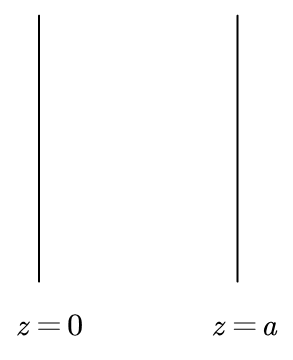
\includegraphics[scale=0.6]{figures/无限大平行板}
	\caption{无限大平行导体板}
	\label{fig:2}
\end{figure}
\paragraph*{}
标量场$\phi$满足Dirichlet边界条件,即
$$
\phi(z=0)=\phi(z=a)=0
$$
两平行板之间单位面积的零点能可以表示为
$$
\mathcal{E} =\frac{\hbar c}{2}\sum_k{\hbar w_k}=\frac{\hbar c}{2}\sum_{n=1}^{\infty}{\int{\frac{d^2k}{\left( 2\pi \right) ^2}\sqrt{k^2+\frac{n^2\pi ^2}{a^2}}}}
$$
式中整数n与横向动量表示板间场的模态。为了计算上式,我们可以使用维度重整化法。假设横向的维度为d,用Schwinger proper-time法表示平方根项:
$$
\mathcal{E} =\frac{\hbar c}{2}\sum_{n=1}^{\infty}{\int{\frac{d^dk}{\left( 2\pi \right) ^d}\int_0^{\infty}{\frac{dt}{t}t^{-1/2}e^{-t\left( k^2+n^2\pi ^2/a^2 \right)}}}}\frac{1}{\varGamma \left( -\frac{1}{2} \right)}
$$
对k积分可得:
$$
\mathcal{E} =-\frac{\hbar c}{4\sqrt{\pi}}\frac{1}{\left( 4\pi \right) ^{d/2}}\sum_{n=1}^{\infty}{\int_0^{\infty}{\frac{dt}{t}t^{-1/2-d/2}e^{-tn^2\pi ^2/a^2}}}
$$
利用Riemann zeta函数,我们可以将零点能表示为:
$$
\mathcal{E} =-\frac{\hbar c}{4\sqrt{\pi}}\frac{1}{\left( 4\pi \right) ^{d/2}}\left( \frac{\pi}{a} \right) ^{d+1}\varGamma \left( -\frac{d+1}{2} \right) \zeta \left( -d-1 \right) 
$$
使用Riemann zeta函数的性质
$$
\varGamma \left( \frac{z}{2} \right) \zeta \left( z \right) \pi ^{-z/2}=\varGamma \left( \frac{1-z}{2} \right) \zeta \left( 1-z \right) \pi ^{\left( z-1 \right) /2}
$$
两平行板间单位面积的零点能可以表示为
$$
\mathcal{E} =-\frac{\hbar c}{2^{d+2}\pi ^{d/2+1}}\frac{1}{a^{d+1}}\varGamma \left( \frac{d+1}{2} \right) \zeta \left( 2+d \right) 
$$
带入d=2,并考虑到横波的两个自由度,可以得到
$$
\mathcal{E} =-\frac{\hbar c \pi ^2}{720}\frac{1}{a^3}
$$
对两平行板间距离求负梯度,我们可以得到单位面积的Casimir力
$$
F_C=-\frac{\hbar c\pi ^2}{240}\frac{1}{a^4}
$$



\section{世界线理论}
粒子在四维时空中的运动轨迹称为世界线。例如一个做自由落体运动的苹果,他在三维空间中的轨迹是一条直线,但在四维时空中的运动轨迹是一个抛物线,因为四维空间中将时间也作为一个坐标轴,如图\ref{fig:4}所示。在量子场论中将场的扰动当作一个粒子,每个粒子都在各自的世界线上运动,运动的时间称为粒子的固有时。
\begin{figure}[h]
	\centering
	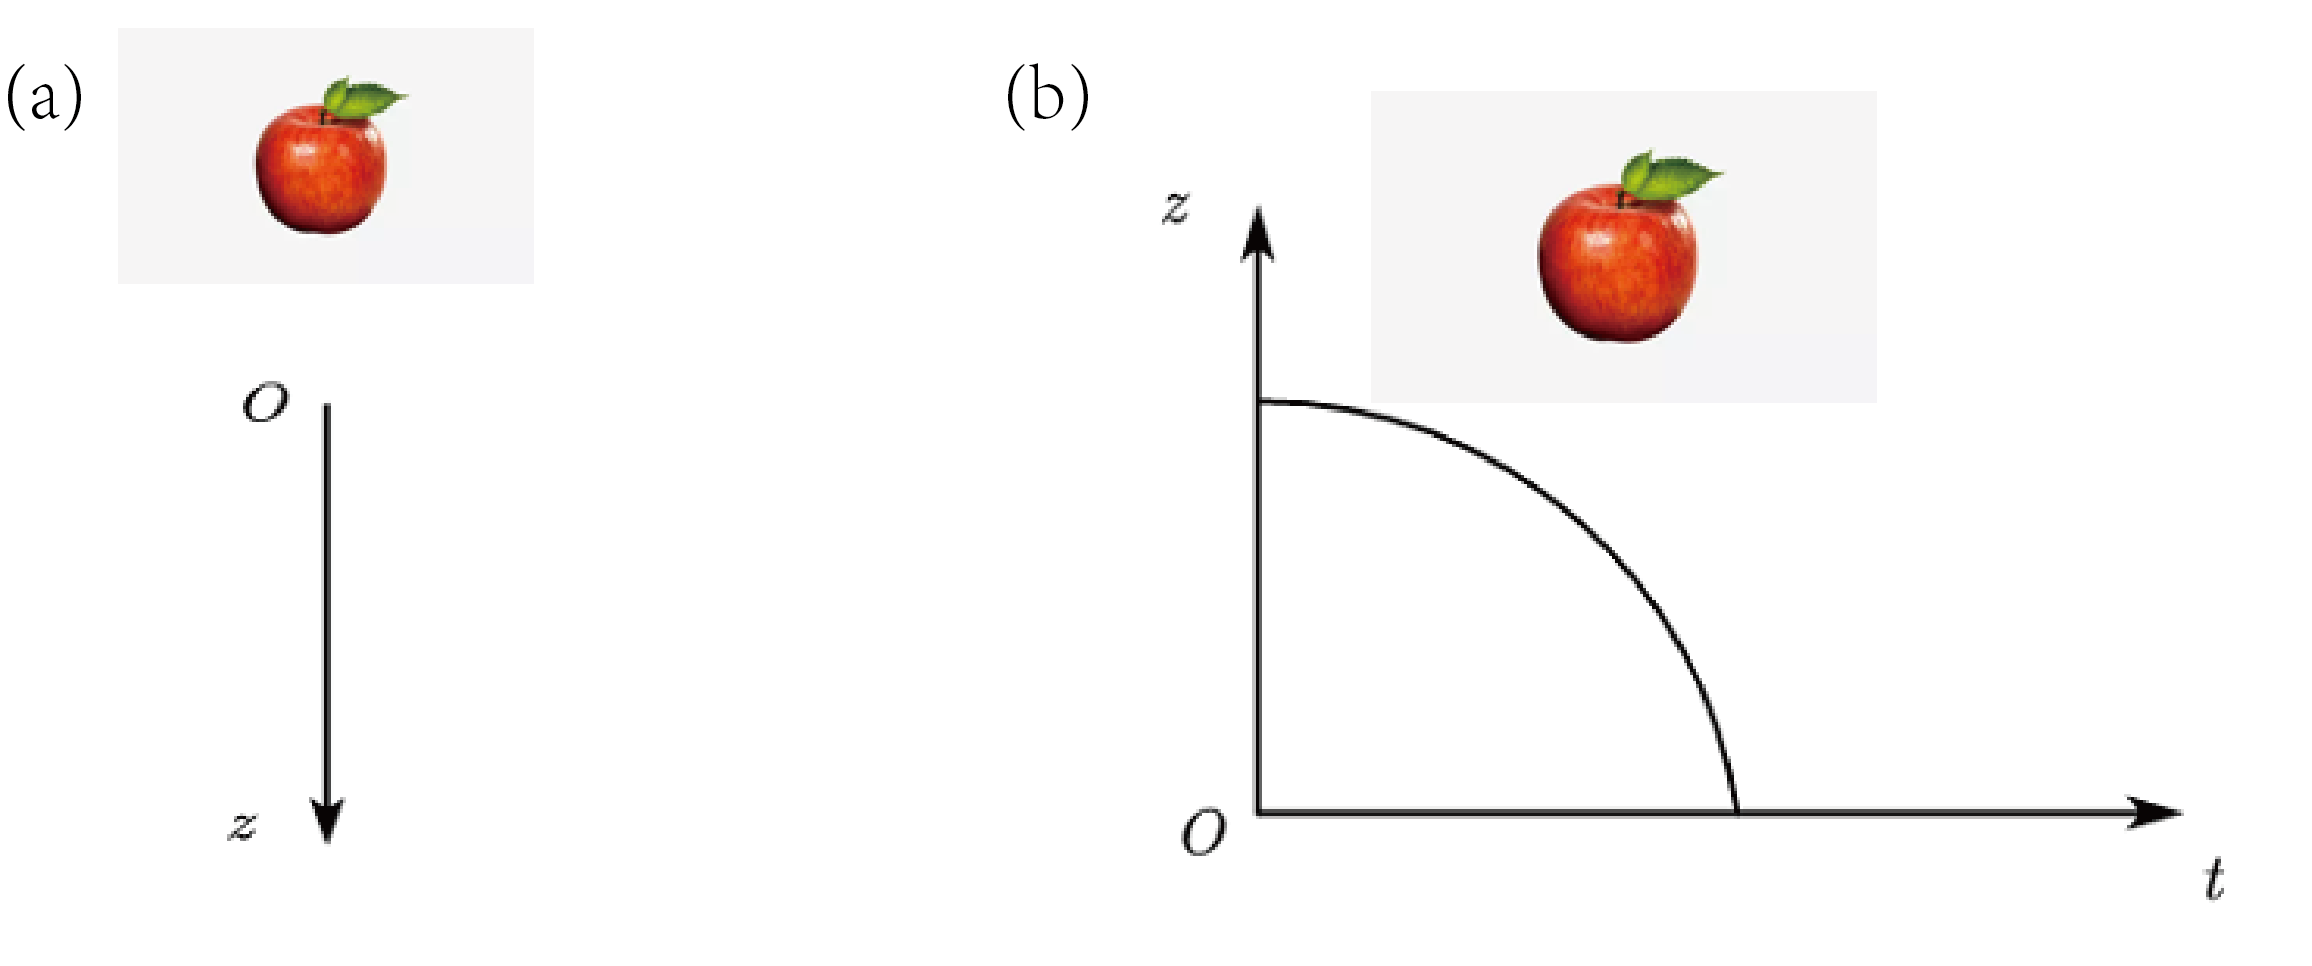
\includegraphics[width=0.7\linewidth]{figures/世界线}
	\caption{世界线示意图(a)苹果在3维空间中的运动轨迹.(b)苹果在4维空间中的运动轨迹}
	\label{fig:4}
\end{figure}
\paragraph*{}
对于一些没有标准几何外形的物体,使用传统的方法(先计算出物体间允许存在的电磁模态,然后将这些模态对应的零点能相加得到总的Casimir能量,再对能量求距离的负梯度得到两物体间的Casimir力)无法计算出物体间的Casimir力,因此2003年Holger Gies 等人提出了世界线方法\cite{Gies_2003,Gies_2006},直接计算电磁模态对应能量的总和。世界线方法的计算很复杂,但是它的物理原理并不复杂,就是将电磁场看作虚拟的粒子,这个粒子在其世界线上运动,运动的总时间为固有时。零点能对应的粒子经过固有时后返回空间原点。如果粒子在三维空间中运动的路径穿过物体的话,便破坏了迪利克雷边界条件,如图\ref{fig:5}(c)所示,也就是说这种粒子对应的是不被允许的电磁模态,需要从系统总能量中删去。这些被删去的电磁模态对应的能量就是两个物体间的相互作用能,即Casimir能。
\begin{figure}
	\centering
	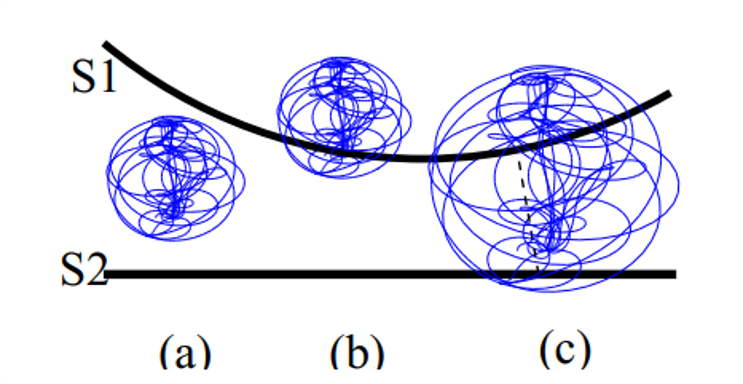
\includegraphics[scale=1]{figures/世界线2}
	\caption{虚拟粒子运动路径与边界的关系(a)未接触(b)穿过一个边界(c)穿过两个边界}
	\label{fig:5}
\end{figure}
用势能V(x)(一般是δ函数的形式)表示两个具有某种几何形状的物体,根据量子场论,和V(x)有关的量子有效作用量为:
$$
\begin{aligned} \Gamma[V] &=\frac{1}{2} \operatorname{Tr} \ln \frac{-\partial^{2}+m^{2}+V(x)}{-\partial^{2}+m^{2}} \\ &=-\frac{1}{2} \int_{1 / \Lambda^{2}}^{\infty} \frac{d T}{T} \int d^{D} x\left[\left\langle x\left|e^{-T\left(-\partial^{2}+m^{2}+V(x)\right)}\right| x\right\rangle-\frac{1}{(4 \pi T)^{D / 2}} e^{-m^{2} T}\right] \end{aligned}
$$
式中D=d+1表示欧式时空维度,d为空间维度,T为固有时,m为场的质量。如果将矩阵元视为量子力学中的跃迁振幅,我们可以将它写成Feynman路径积分(世界线)的形式:
$$
\int d^{D} x\left\langle x\left|e^{-T\left(-\partial^{2}+V(x)\right)}\right| x\right\rangle=\int d^{D} x_{\mathrm{CM}} \mathcal{N} \int_{x(0)=x(T)} \mathcal{D} x e^{-\int_{0}^{T} d \tau \dot{x}^{2} / 4-\int_{0}^{T} d \tau V\left(x_{\mathrm{CM}}+x(\tau)\right)}
$$
在上式中我们把所有闭合路径的中心移到一个公共的质心$x_{CM}$,也就是说$\int_{0}^{T} d \tau x_{\mu}(\tau)=0$,常数$\mathcal{N}$由零势能确定
$$
\left\langle x\left|e^{T \partial^{2}}\right| x\right\rangle \equiv \frac{1}{(4 \pi T)^{D / 2}}=\mathcal{N} \int_{x(0)=x(T)} \mathcal{D} x e^{-\int_{0}^{T} d \tau \dot{x}^{2} / 4}
$$
为了方便数值计算,做变量代换
$$
y_{\mu}(t)=\frac{1}{\sqrt{T}} x_{\mu}(T t) \quad \Longrightarrow \quad \int_{0}^{T} d \tau \dot{x}^{2}(\tau)=\int_{0}^{1} d t \dot{y}^{2}(t)
$$
我们可以得到易于数值计算的量子有效作用量
$$
\Gamma[V]=-\frac{1}{2} \frac{1}{(4 \pi)^{D / 2}} \int_{1 / \Lambda^{2}}^{\infty} \frac{d T}{T^{1+D / 2}} e^{-m^{2} T} \int d^{D} x\left[\left\langle W_{V}[y(t) ; x]\right\rangle_{y}-1\right]
$$
式中
\begin{equation*}
\begin{split}
W_{V}[y(t) ; x]&=\exp \left[-T \int_{0}^{1} d t V(x+\sqrt{T} y(t))\right] \\
\left\langle W_{V}[y(t) ; x]\right\rangle_{y}&=\frac{\int_{y(0)=y(1)} \mathcal{D} y W_{V}[y(t) ; x] e^{-\int_{0}^{1} d t \dot{y}^{2} / 4}}{\int_{y(0)=y(1)} \mathcal{D} y e^{-\int_{0}^{1} d t \dot{y}^{2} / 4}}
\end{split}
\end{equation*}
只要我们计算出势能V(x)对应的量子有效作用量,再除以时间便能得到未重整化的Casimir能$\mathcal{E}=\frac{\Gamma}{L_{x_{0}}}$。因为Casimir力对应的是两个物体间的相互作用Casimir能,如果系统的势能$V(x)$可以分解为$V_1(x)+V_2(X)$,我们可以以将相互作用能定义为
$$
{E} \equiv \varepsilon_{{V}_{1}+{V}_{2}}-\varepsilon_{{V}_{1}}-\varepsilon_{{V}_{2}}
$$
根据之前的分析,我们可以用符合gaubian分布的有限的闭合路径去模拟无穷多的路径\cite{Gies_2001}, gaubian分布概率为
$$
P[\{y(t)\}]=\delta\left(\int_{0}^{1} d t y(t)\right) \exp \left(-\frac{1}{4} \int_{0}^{1} d t \dot{y}^{2}\right),\quad  \quad y(0)=y(1)
$$
首先要将积分离散化,我们一般将路径固有时参数t离散化,即
$$
\{y(t)\} \quad \rightarrow \quad\left\{y_{k}\right\} \in \mathbb{R}^{D},\quad k=1,2,\ldots,N
$$
式中N为每个回路上的点数,由于δ函数的限制,$y_1+ y_2+…y_N=0$。下面介绍一种数值模拟的算法:通过将时间N等分,我们可以将y的微分离散化为
$$
\dot{y} \rightarrow N\left(y_{k}-y_{k-1}\right)
$$
因此有
$$
P\left[\left\{y_{k}\right\}\right]=\delta\left(y_{1}+\cdots+y_{N}\right) \exp \left\{-\frac{N}{4} \sum_{k=1}^{N}\left(y_{k}-y_{k-1}\right)^{2}\right\}
$$
把$y_N=-(y_1+ y_2+…y_{N-1})$带入原方程
$$
\int \mathcal{D} y P\left[\left\{y_{k}\right\}\right] \cdots=\int \prod_{i=1}^{N-1} d y_{i} e^{\left[-\frac{N}{4}\left(\sum_{i=2}^{N-1}\left(y_{i}-y_{i-1}\right)^{2}+\left(2 y_{1}+y_{2}+\cdots+y_{N-1}\right)^{2}+\left(y_{1}+y_{2}+\cdots+2 y_{N-1}\right)^{2}\right)\right]} \ldots
$$
做变量代换
\begin{equation*}
\begin{split}
&\bar{v}_{1} :=\frac{3}{2} y_{1}+y_{2}+y_{3}+\cdots+y_{N-2}+\frac{3}{2} y_{N-1} \\ 
&v_{i} :=y_{i}-y_{i-1},\quad i=2,3,\ldots,N-1 \\
&v_{i,j} =v_{i}+v_{i-1}+\cdots+v_{j+1} \equiv y_{i}-y_{j},\quad for \quad i \geq j=1,2,\ldots,N-1 \\
&\bar{v}_{N-1}:=v_{N-1}+\frac{1}{3} v_{N-2,1}
\end{split}
\end{equation*}
我们可以得到
$$
\int \mathcal{D} y P\left[\left\{y_{k}\right\}\right] \cdots=\bar{J} \int \mathcal{D} \bar{v} \exp \left[-\frac{N}{4}\left(2 \bar{v}_{1}^{2}+\sum_{i=1}^{N-2} \frac{i+2}{i+1} \bar{v}_{N-i}^{2}\right)\right] \cdots \equiv \bar{J} \int \mathcal{D} \bar{v} P\left[\left\{\bar{v}_{k}\right\}\right]
$$
因此我们可以先产生符合分布的$v_i$,然后再转换成$y_i$,具体步骤为\ding{172}先使用Box-muller方法产生N-1个符合$exp(-w_i)$分布的数字$w_i$;
\ding{173}通过如下公式将其转换为$\bar{v}_{i},i=1,\ldots,N-1$
$$
\begin{aligned} \bar{v}_{1} &=\sqrt{\frac{2}{N}} w_{1} \\ \bar{v}_{i} &=\frac{2}{\sqrt{N}} \sqrt{\frac{N+1-i}{N+2-i}} w_{i},\quad i=2,\ldots,N-1 \end{aligned}
$$
\ding{174}再计算$v_i$
$$
v_{i}=\bar{v}_{i}-\frac{1}{N+2-i} v_{i-1,1},\quad \quad v_{i-1,1}=\sum_{j=2}^{i-1} v_{j}
$$
\ding{175}然后产生$y_i$
$$
\begin{aligned} y_{1} &=\frac{1}{N}\left(\bar{v}_{1}-\sum_{i=2}^{N-1}\left(N-i+\frac{1}{2}\right) v_{i}\right) \\ y_{i} &=y_{i-1}+v_{i},\quad i=2,\ldots,N-1 \\ y_{N} &=-\sum_{i=1}^{N-1} y_{i} \end{aligned}
$$
\ding{176}重复上述步骤产生$n_L$个闭合回路。计算物体之间Casimir能的步骤如表\ref{tab:1}所示:
\begin{table}[h]
	\centering
	\caption{使用世界线方法计算Casimir能的步骤}
	\resizebox{\textwidth}{30mm}{
	\begin{tabular}{|r|l|}
		\hline
		\multirow{6}{*}{计算步骤} 
		& 产生$n_L$条符合$\exp \left( -\int\limits_0^1{{dt\dot{y}}^2} \right)$分布的回路 \\ \cline{2-2} 
		& 判断这些回路是否穿过上下极板,如果是,则取$\mathrm{W}_{\mathrm{V}}\left[ \mathrm{y}\left( \mathrm{t} \right) ;\mathrm{x} \right]$为0,否则取1 \\ \cline{2-2} 
		& 计算回路穿过上下极板的概率$<\mathrm{W}_{\mathrm{V}}\left[ \mathrm{y}\left( \mathrm{t} \right) ;\mathrm{x} \right] >$ \\ \cline{2-2} 
		& 对质心x从0到a积分 \\ \cline{2-2} 
		& 对固有时T积分得到量子有效作用量 \\ \cline{2-2} 
		& 将量子有效作用量乘以一个常数得到Casimir能 \\ \hline
	\end{tabular}}
	\label{tab:1}
\end{table}
\paragraph*{}
假设两个平行板间的距离为a,则系统的的势能V(z)为
$$
V(z)=\delta(z-a)+\delta(z)=V_{1}+V_{2}
$$
笔者用python程序模拟了平行板情形,结果如图\ref{fig:6}所示,模拟结果与之前的理论推导结果(Casimir能反比于两个平行板间距离a的三次方)相吻合。
\begin{figure}[h]
	\centering
	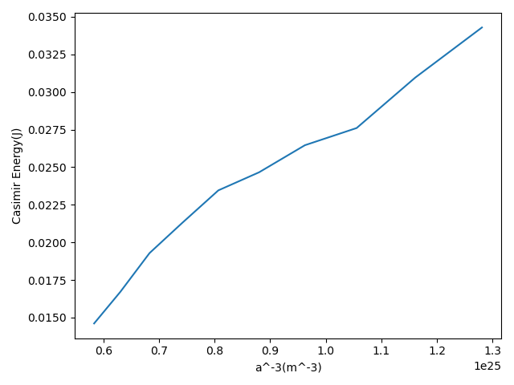
\includegraphics[width=0.7\linewidth]{figures/世界线3}
	\caption{理想导体平行板间单位面积Casimir能与平行板间距的关系}
	\label{fig:6}
\end{figure}



\section{Lifshitz理论}
\paragraph*{}
由于实际的金属都有特定的介电函数,因此研究介质材料间的Casimir效应对于实际应用具有很大的意义。1958年Lifshitz计算出了介电函数以及磁化率对于Casimir效应的影响\cite{Lifshitz_1958}。考虑如图\ref{fig:3}所示的物理模型,左右两平行板均为半无限大的介质板,之间相距$l$。左右平行板以及中间介质的相对介电函数,相对磁化率分别为$\varepsilon _i,\mu _i(i=L,R,m)$。
\begin{figure}[h]
	\centering
	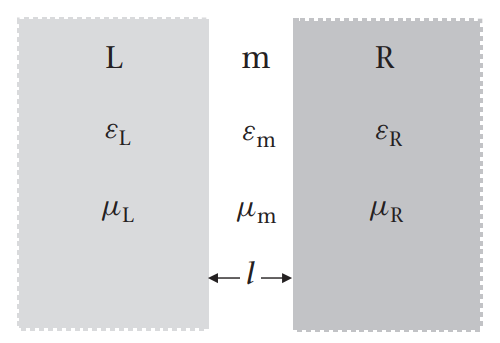
\includegraphics[width=0.7\linewidth]{figures/lifshitz1}
	\caption{平行介质板}
	\label{fig:3}
\end{figure}
\paragraph*{}
假设系统允许存在的电磁场模态为$\{w_j\}$,每种模态对应的能量为:
$$
E_n=(n+\frac{1}{2})\hbar w_j,n=0,1,2\dots
$$
计算每种模态对应的配分函数和吉布斯自由能:
\begin{equation*}
\begin{split}
z(w_j)&=\sum_{n=0}^{\infty}e^{-(n+\frac{1}{2})\hbar w_j/kT}\\
g(w_j) & =-kTln[z(w_j)]\\
& =kTln[2sinh(w_j\hbar/2kT)]
\end{split}
\end{equation*}
只要我们计算出每个模态对应的吉布斯自由能$g(w_j)$,然后对所有的模态求和,就能得到体系的总吉布斯自由能:
$$
G(l)=\sum_{\{w_j\}}g(w_j)
$$
再对极板间的距离求偏导数,便得到平行板间的Casimir力:
$$
F_c=-\frac{\partial G(l)}{\partial l}
$$
下面我们将详细地介绍求解每个模态对应的吉布斯自由能的方法。
\paragraph*{}
存在于介质极板间的电磁场有不同频率的组分,我们可以对其对其做傅里叶展开:
$$\boldsymbol{E}=Re(\sum_{w} \boldsymbol{E}_w e^{-iwt}),\boldsymbol{H}=Re(\sum_{w} \boldsymbol{H}_w e^{-iwt})$$
每一个傅里叶分量 都满足对应的Maxwell方程组:
$$
\begin{cases}
\nabla ^2 \boldsymbol{E}_w +\frac{\varepsilon \mu w^2}{c^2}\boldsymbol{E}_w=0\\
\nabla \cdot \boldsymbol{E}_w=0\\
\nabla ^2 \boldsymbol{H}_w +\frac{\varepsilon \mu w^2}{c^2}\boldsymbol{H}_w=0\\
\nabla \cdot \boldsymbol{H}_w=0
\end{cases}
$$
不妨设垂直于介质表面的方向为z方向,$\boldsymbol{E}$与$\boldsymbol{H}$的各个分量形式为$f(z)e^{i(ux+vy)}$,即:
\begin{equation*}
\begin{split}
E_x&=e_x(z)e^{i(ux+vy)},E_y=e_y(z)e^{i(ux+vy)},E_z=e_z(z)e^{i(ux+vy)}\\
H_x&=h_x(z)e^{i(ux+vy)},H_y=h_y(z)e^{i(ux+vy)},H_z=h_z(z)e^{i(ux+vy)}
\end{split}
\end{equation*}
将电磁场各分量的表达式带入Maxwell方程组的第一和第三个式子,可得:
$$
f''(z)=\rho_i ^2 f(z),\quad \rho_i ^2=(u^2+v^2)-\frac{\epsilon_i \mu_i w^2}{c^2},\quad i=L,m,R
$$
该微分方程的通解形式为:$f_i(z)=A_i e^{\rho_i z}+B_i e^{-\rho_i z}$,且利用电磁场在无穷远处趋于零的条件,有$A_R=0,z>l,B_L=0,z<0$。由$\varepsilon \boldsymbol{E}$ 在z方向的连续性和Maxwell方程组的第二与第四个式子,我们可以得到关于$A_{iz},B_{iz}$的方程组:
$$
\begin{cases}
\varepsilon_L A_{Lz}=\varepsilon_m A_{mz} + \varepsilon_m B_{mz}\\
-A_{Lz}\rho_L=(-A_{mz} + B_{mz})\rho_m\\
\varepsilon_R B_{Rz} e^{-\rho_R l}=\varepsilon_m A_{mz} e^{\rho_m l} + \varepsilon_m B_{mz}e^{-\rho_m l}\\
B_{Rz}\rho_R e^{-\rho_R l}=(-A_{mz} e^{\rho_m l}+ B_{mz}e^{-\rho_m l})\rho_m
\end{cases}
$$
由解的非零性我们可以得出
$$
D_E (w)=1-\frac{\left( \varepsilon _R\rho _m-\varepsilon _m\rho _R \right)}{\left( \varepsilon _L\rho _m+\varepsilon _m\rho _L \right)}\frac{\left( \varepsilon _L\rho _m-\varepsilon _m\rho _L \right)}{\left( \varepsilon _m\rho _R+\varepsilon _R\rho _m \right)}e^{-2\rho _ml}=0
$$
同样的,由磁场的边界条件,我们也可以得出另一个等式
$$
D_H (w)=1-\frac{\left( \mu _R\rho _m-\mu _m\rho _R \right)}{\left( \mu _L\rho _m+\mu _m\rho _L \right)}\frac{\left( \mu _L\rho _m-\mu _m\rho _L \right)}{\left( \mu _m\rho _R+\mu _R\rho _m \right)}e^{-2\rho _ml}=0
$$
定义$D(w) \equiv D_E(w)D_H(w),\rho^2 \equiv u^2+v^2$,则取特定$\rho$的电磁场模态对应的自由能为
\begin{equation*}
\begin{split}
G_l(\rho)&=\sum_{{w_j}}g{(w_j)}
\end{split}
\end{equation*}
然后再对所有$\rho$的积分得到系统的总自由能
$$
G_{LmR}(l)=\frac{1}{(2\pi)^2}Re({\int_{0}^{\infty}2\pi \rho[G_l(\rho)-G_{\infty}(\rho)]d\rho})
$$
其中的系数$1/{(2π)}^2$是因为u,v都随着$w$变化,而$w=2π\nu$,因此$\rho$平面上单位面积内的频率数要乘以$1/{(2π)}^2$。假设$D(w)=\prod_{{w_j}}(w-w_j)$,则根据Cauchy积分定理有
$$
\sum_{\left\{ w_j \right\}}{g\left( w_j \right)}=\frac{1}{2\pi i}\oint_C{g\left( w \right) \frac{d\ln \left[ D\left( w \right) \right]}{dw}dw}
$$
令$w=i\xi $,并代入公式$g(w_j) =kTln[2sinh(w_j\hbar/2kT)]$,经过计算可得
\begin{equation*}
\begin{split}
G_l(\rho)&=\frac{kT}{2}\sum_{n=-\infty}^{\infty}{\ln D\left( i\xi _n \right)}\\
&=kT\sum_{n=(0)1}^{\infty}{\ln D\left( i\xi _n \right)}
\end{split}
\end{equation*}
式中$\xi_n=\frac{2\pi kT}{\hbar}n$,代入计算$G_{LmR}(l)$的公式计算可得
$$G_{\mathrm{LmR}}(l)=\frac{k T}{2 \pi c^{2}} \sum_{n=(0)1}^{\infty} \varepsilon_{\mathrm{m}} \mu_{\mathrm{m}} \xi_{n}^{2} \int_{1}^{\infty} p \ln \left[\left(1-\bar{\Delta}_{\mathrm{Lm}} \bar{\Delta}_{\mathrm{Rm}} e^{-r_{n} p}\right)\left(1-\Delta_{\mathrm{Lm}} \Delta_{\mathrm{Rm}} e^{-r_{n} p}\right)\right] \mathrm{d} p$$
式中$\bar{\Delta}_{\mathrm{ji}}=\frac{s_{\mathrm{i}} \varepsilon_{\mathrm{j}}-s_{\mathrm{j}} \varepsilon_{\mathrm{i}}}{s_{\mathrm{i}} \varepsilon_{\mathrm{j}}+s_{\mathrm{j}} \varepsilon_{\mathrm{i}}},\Delta_{\mathrm{ji}}=\frac{s_{\mathrm{i}} \mu_{\mathrm{j}}-s_{\mathrm{j}} \mu_{\mathrm{i}}}{s_{\mathrm{i}} \mu_{\mathrm{j}}+s_{\mathrm{j}} \mu_{\mathrm{i}}},s_{\mathrm{i}}=\sqrt{p^{2}-1+\left(\varepsilon_{\mathrm{i}} \mu_{\mathrm{i}} / \varepsilon_{\mathrm{m}} \mu_{\mathrm{m}}\right)},r_n = 2l\xi_n\sqrt{\varepsilon_m\mu_m}/c$
考虑介质为真空时的非铁磁性板,有$\mu_{i} \approx 1 \approx \epsilon_{m}, \epsilon_{L}=\epsilon_{R}$,利用PFA近似\cite{Derjaguin_1956,Blocki_1977},我们可以得出半径为R的球和平板之间的Casimir力:
$$
F(z)= \frac{\hbar R}{2 \pi c^{2}} \int_{0}^{\infty} \int_{1}^{\infty} p \xi^{2}\left\{\ln \left[1-\frac{(s-p)^{2}}{(s+p)^{2}} e^{-2 p z \xi / c}\right]\right. \left.+\ln \left[1-\frac{(s-p \epsilon)^{2}}{(s+p \epsilon)^{2}} e^{-2 p z \xi / c}\right]\right\} d p d \xi 
$$




% \section{格林函数法}
% \paragraph*{}
% 我们也可以使用格林函数法推导出平行板间的Casimir相互作用力({\color{red}引用参考书})。一个无质量标量场$\phi$的运动方程可以写成
% $$-\partial^{2}\phi=K,$$
% 对应的格林函数方程可以写为
% $$-\partial^{2}G=\delta(x-{x}').$$
% 对于图2.1(引用图)中的几何,我们可以通过傅立叶变换的方法得到约化格林函数$g(z,{z}')$:
% $$G(x,{x}')=\int \frac{d^{d}k}{(2\pi)^d} e^{i\mathbf{k} \cdot \mathbf{(x-{x}')}}  \int \frac{dw}{2\pi} e^{-iw(t-{t}')}g(z,{z}')$$
% 式中d是横向纬度。约化后的格林函数满足方程:
% $$(-\frac{\partial ^2}{\partial {z}^2}-\lambda ^2)g(z,z')= \delta(z-z')$$
% 式中$\lambda ^2=w^2-k^2$。根据边界条件
% $$g(0,z')=g(a,z')=0$$
% 我们可以算出约化格林函数的表达式为:
% $$g(z,z')=-\frac{1}{\lambda sin(\lambda a)}sin(\lambda a_{<})sin(\lambda (z_{>}-a))$$
% 式中$z_{<}(z_{>})$表示z与z'中较小(大)的那一个数。
% \paragraph*{}
% 我们可以从标量场的能-动量张量计算出边界处的力。对于一个标量场$\phi$,应力张量可以写作:
% $$T_{\mu \nu }=\partial _ {\mu} \phi \partial _ {\nu} \phi +g_{\mu \nu}\mathcal{L} $$
% 式中拉格朗日密度量为$\mathcal{L}=-\frac{1}{2}\partial_{\lambda}\phi \partial^{\lambda}\phi$。根据公式
% $$<\phi(x)\phi(x')>=\frac{1}{i}G(x,x')$$
% 我们可以计算出$T_{\mu \nu }$的期望值。边界处的应力张量常态组分为
% $$<t_{zz}>=\frac{1}{2i}\partial_{z}\partial_{z'}g(z,z')|_{z\to z'=0,a}=\frac{i}{2}\lambda cot(\lambda a)$$
% 我们现在要对上式积分来计算边界处单位面积受力。为了方便积分,我们将坐标进行复频率旋转,
% $$w\to i\zeta,\lambda\to i\sqrt{k^2+\zeta^2}\equiv i\kappa.$$
% 这样的话,单位面积受力可以表示为:
% $$F=-\frac{1}{2}\int \frac{d^{d}k}{(2\pi)^d} \int \frac{d\zeta}{2\pi} \kappa coth(\kappa a)$$
% 但是上式直接计算是发散的,我们假设金属厚度无穷小,这时对应的单位面积受力的表达式为:
% $$F=-\frac{1}{2}\int \frac{d^{d}k}{(2\pi)^d} \int \frac{d\zeta}{2\pi} \kappa (coth(\kappa a)-1)$$
% 使用极坐标表示上述积分:
% $$F=- \frac{{\Omega}_{d+1}}{(2\pi)^{d+1}}\int_{0}^{\infty} \kappa^{d} d\kappa \frac{\kappa}{ (e^{2\kappa a}-1)}$$
% 式中${\Omega}_{d+1}=\frac{2\pi ^{n/2}}{\Gamma(n/2)}$表示d+1为空间对应的球面度。我们利用恒等式
% $$\Gamma(2z)=(2\pi)^{-\frac{1}{2}}2^{2z-\frac{1}{2}}\Gamma(z)\Gamma(z+\frac{1}{2})$$
% $$\int_{0}^{\infty}dy\frac{y^{s-1}}{e^y-1}=\Gamma(s)\zeta(s)$$可以计算出单位面积受力大小为:
% $$F=-(d+1)2^{-d-2}\pi ^{-d/2-1}\frac{\Gamma(1+d/2)\zeta(d+2)}{a^{d+2}}$$
% 带入d=2,有
% $$F=-\frac{\pi ^2}{480}\frac{1}{a^4}$$